\documentclass[en,12pt]{aghdpl}

\usepackage[english]{babel}
\usepackage[utf8]{inputenc}

\usepackage{enumerate}
\usepackage{listings}
\usepackage{caption}
\usepackage{subcaption}
\usepackage{verbatim}
\usepackage{booktabs}
\usepackage{mathtools}
\usepackage{textcomp}
\usepackage{amssymb}
\usepackage[table,xcdraw]{xcolor}
\usepackage{siunitx}
\usepackage{hyperref}
\usepackage{float}
\lstloadlanguages{TeX}

\lstset{
  literate={ą}{{\k{a}}}1
           {ć}{{\'c}}1
           {ę}{{\k{e}}}1
           {ó}{{\'o}}1
           {ń}{{\'n}}1
           {ł}{{\l{}}}1
           {ś}{{\'s}}1
           {ź}{{\'z}}1
           {ż}{{\.z}}1
           {Ą}{{\k{A}}}1
           {Ć}{{\'C}}1
           {Ę}{{\k{E}}}1
           {Ó}{{\'O}}1
           {Ń}{{\'N}}1
           {Ł}{{\L{}}}1
           {Ś}{{\'S}}1
           {Ź}{{\'Z}}1
           {Ż}{{\.Z}}1
}

\usepackage{tikz}
\usetikzlibrary{arrows,automata,shapes,positioning,shadows,trees}

%---------------------------------------------------------------------------

\author{Jakub Olesiński}
\shortauthor{J. Olesiński}

\titlePL{Rozpoznawanie obiektów na obrazach RGB-D  pod kątem zastosowań w robotyce}
\titleEN{Object recognition in RGB-D images for robotic applications.}

\shorttitlePL{Object recognition in RGB-D images for robotic applications.}
\shorttitleEN{Object recognition in RGB-D images for robotic applications.}

\thesistype{Praca dyplomowa magisterska}
\thesistypeEN{Master of Engineering Thesis}

\supervisor{dr inż. Paweł Rotter}

\degreeprogramme{Automatyka i Robotyka}
\degreeprogrammeEN{Automatics and Robotics}

\date{2017}

\department{Katedra Automatyki i Inżynierii Biomedycznej}
\departmentEN{Department of Automatics and Biomedical Engineering}

\faculty{Wydział Elektrotechniki, Automatyki,\protect\\[-1mm] Informatyki i Inżynierii Biomedycznej}
\facultyEN{Faculty of Electrical Engineering, Automatics, Computer Science and Biomedical Engineering}

\acknowledgements{}


\setlength{\cftsecnumwidth}{10mm}

%---------------------------------------------------------------------------
\setcounter{secnumdepth}{4}

\begin{document}

\titlepages
\setcounter{tocdepth}{3}
\tableofcontents
\clearpage

%\chapter*{Introduction}
\markboth{Introduction}{Introduction}
\label{cha:introduction}
\addcontentsline{toc}{chapter}{Introduction}  

%---------------------------------------------------------------------------

% Aim - 
% Contents -

The aim of this work is to survey modern RGB-D image processing algorithms for model-based object recognition. Analysis of each method is focused on their usability in time and resource constrained robotic environment. Based on provided performance evaluation, selected methods are used to develop a complete, applicable in robotics, object recognition system.

The first chapter provides project background. A formal problem statement is included and followed by categorized solution proposals found in literature, outlining the scientific context of this work. The RGB-D imaging basics are subsequently introduced, together with software tools and test environment utilized throughout the project.

Second chapter introduces preprocessing techniques. Firstly, different data representation and conversion methods are discussed. Basic depth processing operations are introduced afterwards, including spatial transformations, neighbourhood selection and normal estimation. Different noise types encountered in RGB-D images and their corresponding filtering methods are further discussed.

Model fitting with sparse feature matching algorithms is presented in chapter three. Selected keypoint detectors and descriptors of both color and shape modalities are compared and an efficient matching technique is provided. Further, correspondence clustering and pose estimation methods are evaluated.
% Pose estimation may go into postprocessing

The following chapter is about 

%Model fitting algorithms are presented in chapter three. Performance of data alignment and correspondence matching methods is tested together with different descriptor approaches. Statistical methods of result verification are finally presented and used to test the complete object recognition system.

%Chapter four generalizes models from previously developed approach into categories. A neural network approach is presented as a data classifier. Convolutional neural network architecture is proposed and its implementation, training and performance tests are provided.

%The last chapter describes several application scenarios of the developed system. Here should be placed one sentence per scenario. Here should be placed one sentence per scenario. Here should be placed one sentence per scenario. Each tested against different noise conditions.

% 1st - RGB-D basics. Basics, Background, Problem background, Project backgrount, Project settlement, FIND EXAMPLE INTRODUCTIONS
%% Includes: color + depth intro, depth acquisition, work environment: software, hardware and datasets, and related work (pipelines).
% 2nd - Preprocessing
%% Includes: representation, neighbourhood, viewpoint transformations, noise filtering, segmentation, keypoint detection
% 3rd - Recognition
%% Includes: Alignment methods, matching, descriptors, hypothesis verification
% 4th - Classification
%% Includes: Convolutional neural network, training, tests
% 5th - Applications
%% Includes: Scenarios with simulation

\chapter{Introduction}
\label{cha:introduction}

The aim of this work is to survey modern RGB-D image processing algorithms for model-based object instance recognition. Each method is analyzed with focus on its employment in time and resource constrained robotic environment. Based on provided performance evaluation, selected methods are used to develop a complete, applicable in robotics, object recognition system.

The first chapter provides project background. A formal problem statement is followed by a brief literature review, introducing the main categorization of solution proposals into feature and template matching techniques. After outlining the scientific context of this work, software libraries and tools for RGB-D image processing used throughout the project are presented. Algorithm evaluation methodology, reference dataset and hardware used for performance assessment are summarized at the end of this chapter.

Second chapter introduces common pre-processing techniques for RGB-D images. At first, different data representation and conversion methods are discussed. Fundamental concepts in further processing, including neighborhood selection and surface normal estimation are introduced and evaluated afterwards. To finalize this chapter, different noise types encountered in RGB-D data are discussed together with their corresponding filtering methods.
 
Model fitting with sparse feature matching algorithms is presented in chapter three. Selected keypoint detectors and descriptors of both color and shape modalities are compared. Efficient matching technique is provided. Correspondence clustering. Pose estimation methods are evaluated.

Template matching methods are discussed in the following chapter. Global features. Linemod. Bag of words. Neural networks.

Postprocessing. Pose refinement. Hypothesis verification.

Applications.

%---------------------------------------------------------------------------

\section{Problem statement}
\label{sec:problem}

%TODO: division to category/instancem from Szelski 14.3
Broad topic, \cite{szeliski}.

Given an input image and an object of interest, the task of object recognition is to provide answer to the following questions:
\begin{itemize}
\item Is the queried object \textit{present} in the image?
\item If it is, then what is the \textit{pose} of the object?
\end{itemize}
If the object has the properties of a rigid body, its pose is given by the linear and angular position.


Object recognition is a process that comprises determination of both object instance presence and its pose in a given scene image.   

Robotics: why object recognition
Object recognition: why RGB-D

%% methods of depth acquisition
%% applications in robotics, mapping, 3d modeling


%---------------------------------------------------------------------------

\section{Related work}
\label{sec:related}

%look for similar cotributions
%survey (in robotics): if nothing may be descr/keypoints comparison
%generic, open source system: mention ORK, V4R etc

Survey of local methods \cite{surveyLocal}.
Pipelines \cite{recognitionTutorial,multiPipeline}.

%---------------------------------------------------------------------------

\section{Software tools}
\label{sec:software}

Throughout this work, most of the software was developed with an extensive use of the Point Cloud Library (PCL)\cite{Rusu_ICRA2011_PCL}, which is an open source C++ library for three dimensional image processing. Since 2011, it is developed by a large scientific community, maintained by the Open Perception foundation and delivered under BSD license. PCL provides implementations of a multitude of novel algorithms for 3D filtering, feature estimation, segmentation, registration and model fitting, together with tools for visualization and camera interfacing.

The Open Computer Vision (OpenCV)\cite{OpenCV} library was utilized as another source of implementation for the analysed algorithms. OpenCV, which is a more mature project, developed since 1999 is likewise delivered under open source BSD license. While PCL is mainly focused on volumetric data analysis, OpenCV provides a wide array of functions for 2D intensity and color image processing.

Modeling \cite{modellingV4R}
V4R \cite{multiPipeline}
% ROS
% Ecto

%---------------------------------------------------------------------------

\section{Test environment}
\label{sec:testhardware}

Timing perf hardware

Testing of implemented algorithms was done on two hardware platforms: an embedded computing board NVidia Jetson TK1 and personal laptop Lenovo Y50-70. Parameters of both computers are summarized in table [x]. 

\begin{table}[H]
\centering
\begin{tabular}{r c | c}
& NVidia Jetson TK1 & Lenovo Y50-70 \\ 
 \hline
 CPU:& ARM Cortex-A15 2.32GHz x4 & Intel Core i7-4720HQ 2.60GHz x4\\
 GPU:& NVIDIA Kepler GK20a & NVidia GeForce GTX 960M \\
 &with 192 SM3.2 CUDA cores& with 640 SM5 CUDA Maxwell cores\\
 &(upto 326 GFLOPS)&(upto xx GFLOPS)\\
 RAM:& 2GB DDR3L 933MHz 64 bit&  16GB DDR3L 1600MHz (4GB GPU 2.5Mhz 128bit)
\end{tabular}
\caption{Test hardware specification}
\label{tab:hardware}
\end{table}

Dataset Willow

Recognition system was validated against sample dataset from XXX, which provides full object models together with real world scene scans and ground truth position annotations. To 

% Multimodal blending sec. 3

%TODO:
Dataset own using V4R and Xtion sensor

% TODO:
Precision vs Recall, ROC curves from Szelski

%---------------------------------------------------------------------------
% 2nd - Preprocessing
%% Includes: representation, neighbourhood, viewpoint transformations, noise filtering, segmentation, keypoint detection
\chapter{Pre-processing}
\label{cha:preproc}

This chapter describes basic RGB-D image processing tool set, that prepares an input image for extracting relevant information during object recognition.

%---------------------------------------------------------------------------

\section{Representation}
\label{sec:representation}


%rgb-d, point clouds, tsdf
%algos for conversion, timing

Depth and colour information of the environment can be represented in computer memory by the means of various data structures, which differ in their complexity and applicability. In case of typical, low-cost RGB-D cameras, the raw data that is retrieved from the device firmware and operating system drivers come in a form of two images, one from a conventional colour camera and the other from the depth sensor, as depicted on Figure x.

Figure XXX - drawing of camera with 2 raycasts, 2 images

Data retrieved from a depth sensor have a form of one channel, two dimensional image. Each pixel contains measurement of the distance between depth camera reference frame origin and a corresponding point on the reflected surface. In case of Asus Xtion sensor, this data is stored as 32 bit floating point values. It is important to note, that depending on the acquisition method, not all of the surface point distances are measured. For example, if the surface is translucent, most sensors will fail to retrieve proper distance. Such situation is reflected in data by the use of \textit{Not a Number (NaN)} pixel values.

Due to the displacement between color and depth sensor [reference], RGB-D cameras require a calibration step to align the measurements. For this purpose, open source packages such as [XXX] can be used. Finally, successful RGB-D data alignment yields a four channel digital image, which can be defined more formally as:
\begin{equation}
\label{eq:rgbdimage}
I: \{1,\dots,M\} \times \{1,\dots,N\} \rightarrow [0,1]^4,\qquad I(u,v) =  \begin{bmatrix} I_R(u,v) \\ I_G(u,v) \\ I_B(u,v) \\ I_D(u,v) \end{bmatrix},
\end{equation}
where:
\begin{itemize}
\item $M \in \mathbb{N}$, $N \in \mathbb{N}$ - row and column image size,
\item $I_R(u,v), I_G(u,v), I_B(u,v)$ - red, green and blue colour channel intensities,
\item $I_D(u,v)$ - depth channel intensity
\end{itemize}

RGB-D image formulation \ref{eq:rgbdimage} is mostly suitable for per channel, classic two-dimensional image processing, such as applying morphological operators or linear filters [XXXImProc]. It does, however, limit the three dimensional surface information to a single viewpoint, which is undesirable for some applications in robotics, especially for object modelling and environment mapping. A generalized data representation that overcomes this limitation is called a \textit{point cloud}. It can be defined as a point set $C \subset \mathbb{R}^N$ of $N$-dimensional vectors. Depending on the usage, the points can represent different image modalities and features, such as point location in some reference frame, colour, surface normal vector or more advanced descriptors (see chap. \ref{cha:feature}). Direct conversion from a depth map to point cloud, requires projective transformation [XXX] of the depth channel to render Cartesian $x,y,z$ point coordinates in camera reference frame. In this manner, multiple RGB-D image frames, taken from different viewpoints can be stored within a single point cloud, by registering their points to a common coordinate system.

There are other possible representations of depth data. In contrast to point clouds, \textit{Patch volumes} [XX] and \textit{Signed distance functions} are dense representations of the three-dimensional environment, where each point represents distance to the nearest surface. Patch volumes use BLABLABLA. OctoMaps use BLABLABLA. Those representations, however, are mainly used for environment mapping and SLAM applications. This work will further focus on point clouds, as they are the most covered representation for object recognition. ??

%TODO: model format

%---------------------------------------------------------------------------

\section{Neighbourhood}
\label{sec:neighbourhood}

Similarly to classical image processing, a wide range of point cloud processing algorithms rely on the notion of point neighbourhood. Given a metric function $d$ and a query point $p_q$ in the point cloud $P$, two commonly used types of neighbourhoods can be defined. A \textit{r-neighbourhood} is a set composed of all the points $p_i \in P$ that lie within a sphere of a radius $r$ and a center in $p_q$, thus satisfying the condition
\begin{equation}
d(p_	q, p_i) \leq r.
\end{equation}
The other type is \textit{k-neighbourhood}, a set of $k$ nearest points in the sense of given metric. Proper determination of neighbourhood size parameters, either $r$ or $k$ correspondingly, is crucial in further analysis. Too small values do not provide enough information about the surface. Too large, on the other hand, will average the surface and skip small details. Complexity and efficiency of neighbourhood search depends on different internal data representation in a point cloud.

From computational point of view, a point cloud that is directly converted from RGB-D image can be internally stored in a two dimensional array of points, with elements corresponding to image pixels. Point clouds with such data arrangement are commonly referred to as \textit{organized}. Image-like ordering is beneficial, because it reflects the spatial distribution of points directly into memory.


Also known as support.
Organized neighbourhoods.
KD-tree.
Flann.
\textit{“scale” corresponds to the “support radius” (TombariA et al, 2013)}
%---------------------------------------------------------------------------

\section{Surface normals}
\label{sec:normals}

Many of the algorithms used further during the analysis of a point cloud base on the notion of a surface normal, known from the 3D geometry. These vectors are also widely used for shading in 3D computer graphics and a variety of methods have already been developed to solve the surface normal estimation problem. One of the simplest uses the least-squares plane fitting to estimate the normal to a plane tangent to the surface, which approximates the desired vector \cite{rusuthesis}. More specifically, for a given point on the surface, it's $k$-neighbourhood centroid $\bar{p}$ is calculated as:
\begin{equation} 
\bar{p} = \frac{1}{k} \cdot \sum\limits_{i=1}^{k} p_i 
\end{equation}
The tangent plane is thereafter defined by the centroid $\bar{p}$ and the sought normal vector $\vec{n}$. The latter is computed by minimizing the total distance from every k-neighbour $p_i$ to the tangent plane, given by $\sum\limits_{i=1}^{k} (p_i - \bar{p})\cdot \vec{n}$. The minimization problem can be solved by utilizing the covariance matrix $C \in \mathbb{R}^{3x3}$, given by:
\begin{equation}
C = \frac{1}{k-1}\sum\limits_{i=1}^{k}(p_i - \bar{p})\cdot (p_i - \bar{p})^\intercal
\end{equation}
The covariance matrix $C$ is symmetric, positive semi-definite and possess three real eigenvalues $\lambda_j \geq 0, i = 1,2,3$. The eigenvector corresponding to the smallest eigenvalue is an approximation of the desired normal vector $\vec{n}$, disregarding the sign. Furthermore, if the viewpoint $v_p$ is known, the normal $\vec{n}$ has to be oriented towards  $v_p$, which means that it has to satisfy the condition:
\begin{equation}
\vec{n}\cdot(v_p-p_i) > 0
\end{equation}


Processing time. Cuda implementation. Complete solution used \cite{eigenvalues3x3}.

Example PCD with normals:
\begin{figure}[h]
\centering
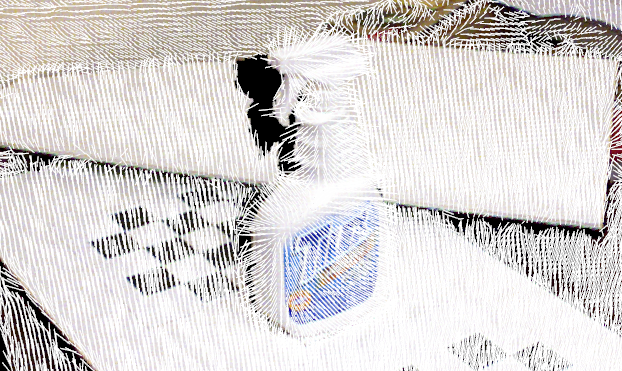
\includegraphics[width=0.8\textwidth]{fig/Normal}
\caption{ Normals }
\label{fig:normals}
\end{figure}

\section{Noise filtering}
\label{sec:noise}

%TODO: types of noise
Types of noise, frequency response, low pass filtering, nonlinear filtering

%TODO: boundary
Boundary estimation

%TODO: clutter
Occlusion and clutter from Guo

One of the most important stages of data preprocessing is the filtration. Probably the most basic point cloud filter is the pass-through filter, which reject all points outside a given range along a specified dimension. This procedure allows to focus the analysis process on the region of interest, i.e. the reachable workspace of a manipulator. Apart from limiting the cloud dimensions, the number of data points can be also reduced by downsampling. The voxel grid filter is typically used for this purpose. This filter creates a three dimensional regular grid over the input point cloud data and then, in each voxel, approximates all the present data points with their centroid. Such reduction is particularly useful when large point cloud datasets have to be processed online with limited computing resources. Finally, the filtration process has to cope with numerous measurement errors present in the raw data acquired from the 3D camera. Such measurement noise 
manifests itself in the form of sparse outliers, which corrupt the results of further processing, i.e. the surface normals estimation. The impact of those irregularities can by reduced by applying an outlier removal filter. The simplest form of such filter rejects all the data points which does not have enough neighbours within a specified radius. A more refined version is based on the neighbouring points distance distribution. Firstly, the mean distance from each point to all its neighbours is calculated. Next, based on the assumption that the resulting distribution is Gaussian, all the points whose mean distances lay outside of an interval defined by the global distances mean and their standard deviation are rejected from the dataset. The effects of statistical outlier removal are presented in the Figure \ref{fig:outlierremoval}.

%---------------------------------------------------------------------------

% 3rd - Recognition
%% Includes: Alignment methods, matching, descriptors, hypothesis verification

\chapter{Sparse feature matching}
\label{cha:feature}

Solutions to problem stated in section \ref{sec:problem} are commonly divided \cite{something} into feature-based and template-based. The former approach, also referred to as local matching, is focused on comparing point neighbourhoods between the scene and model datasets. 

The solution in such methods is composed of several steps. Firstly, an input subset with elements of rich and distinguishable neighbourhood information is selected. Points that belong to this subset are referred to as \textit{keypoints}. For each keypoint, its neighbourhood information is expressed in the form of a \textit{descriptor} vector. By the means of selected metric, commonly the $L_2$ norm, descriptors are further compared between the scene and model datasets, to find \textit{correspondences} with minimal distance. Such point pairs are then grouped to share similar geometric constrains and finally, the largest clusters are used to calculate affine transformation, which renders the initial problem solution.

The inherent locality of feature matching methods has direct implications on the solution performance. Such methods are by design robust to occlusions \cite{something}. Each point is processed independently, which enables data parallelization to boost time performance. Conversely, keypoint identification requires costly analysis of the whole input dataset, thus a balance between the recognition performance and time effectiveness is required \cite{somethin} for real-time applications.

%---------------------------------------------------------------------------

\section{Shape description} %SHOT}
\label{sec:shape} %shot}

There is a multitude of proposals for shape key-point detectors existing in literature. An overview and performance evaluation of the most popular methods can be found in \cite{keypoints1} and \cite{keypoints2}. From both evaluations, the \textit{Intrinsic Shape Signatures} (ISS) \cite{ISS} detecor is worth particular attention. \cite{keypoints1} states that ISS, as a fixed-scale detector, copes well with full three-dimensional models and provides a proper balance between the repeatability rate and time efficiency. In \cite{keypoints2}, the ISS is evaluated with the best repeatability rate among detector implementations available in PCL. The ISS introduces a saliency measure, defined by the smallest eigenvalue of the neighbourhood scatter matrix. For a given point $p$ and its neighbourhood $N$, the scatter matrix $\Sigma$ is given by
\begin{equation}
\label{eq:scatter}
\Sigma(p,N) = \frac{1}{|N|} \sum\limits_{q\in N}(q -\mu_p)(q - \mu_p)^T,\ \mu_p = \frac{1}{|N|}\sum\limits_{q\in N}q
\end{equation}
% originally defined as weighted matrix, need to check how its implemented
By denoting the eigenvalues of $\Sigma(p, N)$ as $\lambda_1 > \lambda_2 > \lambda_3$, the ISS detector classifies $p$ as a keypoint, if the following condition is satisfied
\begin{equation}
\label{iss}
\frac{\lambda_2}{\lambda_1} < \epsilon_1 \  \land \  \frac{\lambda_3}{\lambda_2} < \epsilon_2 \ \land \  \lambda_3 > \epsilon_3.
\end{equation} 
Thresholds $\epsilon_1$ and $\epsilon_2$ are meant to provide sufficient difference between variations along each principal direction, which aids in estimation of a repeatable reference frames for further description stages. The third threshold $\epsilon_3$ ensures that the variations are large enough to consider the point as interesting. A further improvement to the ISS detection criteria is to apply non-maximum suppression over the saliency measure computed at each point. With this edge thinning technique, a point is classified as a keypoint, if it has the largest $l_3$ over its neighbourhood.  An example of keypoints detected with ISS is presented on figure \ref{fig:iss}. The object (cleaning spray in the center of the figure) has marked points in areas of rich shape information, like the bottleneck or the nozzle. It is also visible, that ISS classifies wrong points in two cases. Firstly, when a point lies on a visibility boundary (i.e. the edges of flat surfaces in the figure), thus it should be extended with boundary detection as described in xx. Secondly, when the sensor noise is high (distant wall flat surface in upper left edge of the figure). This issue can be handled by ignoring points above certain z-distance from the sensor or by adaptatively selecting neighbourhood radius for saliency measure.
%select rich shape object from willow = 13
%implement hardload and iss, measure avg time
%implement in cuda

\begin{figure}[h]
\centering
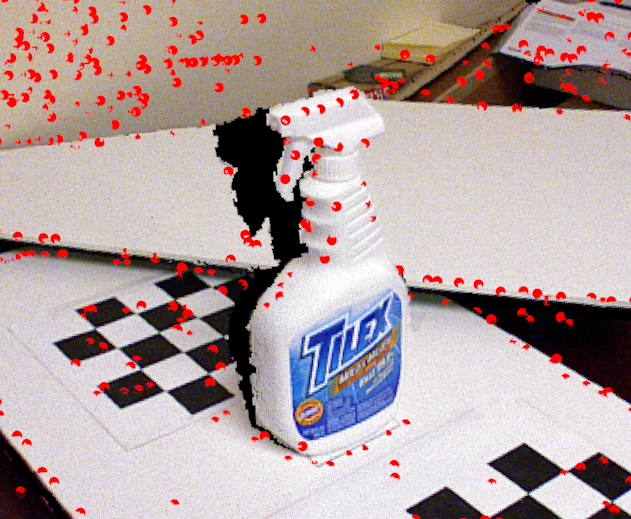
\includegraphics[width=0.8\textwidth]{fig/ISS}
\caption{ISS keypoints (marked with red) computed with $\epsilon_1 =  \epsilon_2 = 0.75$ and $\epsilon_3 = 0.0005$ }
\label{fig:iss}
\end{figure}

The overall time complexity of ISS classification is at the order of $O(nk)$, where $n$ is the image size and $k$ is the max neighbourhood size. This translates into average execution times on target platforms, provided in table \ref{tab:issexec}.

\begin{table}[h]
\centering
\begin{tabular}{r || c | c}
& NVidia Jetson TK1 & Lenovo Y50-70 \\
 \hline
 \hline
 PCL ISS& 4s & 4s \\
 PCL ISSBD& 4s &  4s \\
 CUDA ISS& 4s & 4s \\
 CUDA ISSBD& 4s & 4s
\end{tabular}
\caption{ISS detector time performance statistics.}
\label{tab:issexec}
\end{table}

It is important to note, that in practical applications the keypoint detection step is often replaced by volumetric down sampling. About voxel grid. Model is densely grained. This avoids computational costs of keypoint detection, but increases the complexity of further matching and clustering stages. How to choose this tradeoff.
%In \cite{keypoints-learning}, authors propose a random-forest classifier to be trained for detection of the best interest points for any chosen descriptor.

%Provide complexity, measure time perf (and invariance to transformations?). Can be skipped with uniform.

Descriptor comparison. Take SHOT \cite{SHOT}. Complexity, time perf. Extension with color. \cite{CSHOT}

%----------------------------	-----------------------------------------------

\section{Texture description} %ORB}
\label{sec:colour} %orb}

matching \cite{ORB}

%---------------------------------------------------------------------------

\section{Clustering}
\label{sec:clustering}

geometric consistency, hough

%---------------------------------------------------------------------------

\section{Alignment}
\label{sec:alignment}

umeyama, ransac


% 4th - Classification
%% Includes: Convolutional neural network, training, tests

\chapter{Verification}
\label{cha:verification}

%---------------------------------------------------------------------------

\section{Pose refinement}
\label{sec:icp}

icp

%---------------------------------------------------------------------------

\section{Global hypothesis verification}
\label{sec:ghv}

ghv, ghv from v4r
% 4th - Classification
%% Includes: Convolutional neural network, training, tests

\chapter{Post-processing}
\label{cha:postproc}

%---------------------------------------------------------------------------

\section{Pose refinement}
\label{sec:icp}

icp

%---------------------------------------------------------------------------

\section{Hypothesis verification}
\label{sec:ghv}

ghv, ghv from v4r

multi pipeline
% 5th - Applications
%% Includes: Scenarios with simulation

\chapter{Applications}
\label{cha:applications}

%---------------------------------------------------------------------------

\section{Scenario 1}
\label{sec:scenario1}

something simple with recognition
object retrieval in robot environment

simulation of something simple

%---------------------------------------------------------------------------

\section{Scenario 2}
\label{sec:scenario2}

something simple with classification
object following

simulation of something simple

%---------------------------------------------------------------------------

\section{Scenario 3}
\label{sec:scenario3}

Robocup@Work

simulation of Robocup@Work?

%---------------------------------------------------------------------------

\section{Scenario 4}
\label{sec:scenario4}

APC?

Synthetic dataset from APC gazebo.
simulation of APC?
%https://arxiv.org/pdf/1509.01277.pdf
%http://pracsyslab.org/rutgers_apc_rgbd_dataset
%---------------------------------------------------------------------------
\chapter*{Summary}
\label{cha:summary}
\markboth{Summary}{Summary}
\addcontentsline{toc}{chapter}{Summary}  

% Results -
% Conclusions -
% Future -

\bibliographystyle{ieeetr}
\bibliography{bibliography}

\end{document}
